% ============================================================================
\section{Evaluación empírica del optimizador}
\label{sec:evaluacion}
% ============================================================================

Esta sección mide el optimizador contra un óptimo exacto y contra varias
líneas base. La pregunta de fondo es si la complejidad del NSGA-II se
justifica: si una alternativa más simple ---una regla voraz o un modelo de
decisión de propósito general--- arma kits igual de buenos, el NSGA-II sería
complejidad sin retorno.

\subsection{Diseño experimental}

\paragraph{Instancias.} Las 175 listas oficiales del corpus (17 colegios,
todos sus grados) pasaron por la misma normalización y resolución del sistema
(\cref{sec:normalizacion,sec:resolucion}) contra una foto fija del catálogo
(135 conceptos, 684 productos). Una lista no tiene ninguna línea decidible, así
que quedan 174 instancias. En promedio, una instancia tiene 17 líneas
decidibles con 2,4 candidatos por línea (máximo 3). En 137 de las 175 listas
$\card{\Esp}>4096$ y el NSGA-II se ejecuta; en las demás se enumera el frente
exacto. La resolución usó solo el canal léxico, porque la cuota del modelo de
\emph{embeddings} se agotó durante la generación de las instancias. Esto no
afecta la comparación, porque todos los competidores reciben exactamente los
mismos candidatos.

\paragraph{Escenarios.}
\begin{itemize}
  \item \textbf{Ahorrador}: el kit más barato (174 listas).
  \item \textbf{Premium}: la mejor marca posible (174 listas).
  \item \textbf{Fan}: el personaje más frecuente de la lista, al menor costo
        (157 listas; 17 no tienen ningún producto con personaje).
  \item \textbf{Presupuesto}: la mejor marca que cabe en un tope fijado en la
        mitad del camino entre el kit más barato y el Premium (174 listas).
\end{itemize}

\paragraph{Referencia exacta.} Por la \cref{prop:separable}, los tres primeros
escenarios se resuelven exactamente línea por línea
(\cref{cor:extremos}), y el de presupuesto con la programación dinámica del
\cref{teo:mckp-poli}. La implementación de referencia se verificó contra
fuerza bruta con 27 pruebas.

\paragraph{Competidores.}
\begin{enumerate}
  \item \emph{NSGA-II (producción)}: el procedimiento de la
        \cref{sec:opt-completo} en su versión v3, con cinco semillas.
  \item \emph{NSGA-II, mejor punto del frente}: solo en el escenario de
        presupuesto, el punto del frente de mayor fidelidad que cabe. Mide lo
        que el optimizador ya calculaba y la recomendación no entregaba.
  \item \emph{Regla simple}: la heurística por perfil
        (\cref{def:heuristica}) en su versión de entonces, que ordenaba por
        precio unitario.
  \item \emph{Kits de reglas con juez perfecto}: cinco kits armados con reglas
        simples y un selector que siempre acierta. Separa la calidad de un
        conjunto de kits de la calidad de quien elige entre ellos.
  \item \emph{Modelo de decisión de propósito general}: un modelo abierto de
        421 millones de parámetros, diseñado para tomar decisiones
        tipificadas a partir de texto, probado en cuatro modalidades: (A) una
        pregunta por línea, (B) la lista completa como contexto, (C) decisión
        secuencial con el presupuesto restante y (D) juez entre los cinco kits
        de reglas. La versión y el formato de pregunta se eligieron en una
        prueba de cordura previa con 200 casos sintéticos, \emph{antes} de ver
        las instancias.
  \item \emph{Azar}: un candidato al azar por línea.
\end{enumerate}

\paragraph{Métricas.} Porcentaje de listas en que el kit iguala el óptimo;
sobrecosto medio (Ahorrador); fidelidad perdida (Premium); personaje logrado
(Fan); en presupuesto, si cabe y qué fracción de la fidelidad óptima logra.
Además, el porcentaje de listas en que el kit está \emph{dominado por el
frente}, es decir, en que algún punto del frente del NSGA-II es igual o mejor
en los cuatro objetivos y estrictamente mejor en alguno.

\subsection{Resultados}

\begin{table}[htbp]
\centering\small
\caption{Resultados por escenario (versión v3 del optimizador). «Iguala»:
porcentaje de listas en que el kit es el óptimo. «Dominado»: porcentaje en que
algún punto del frente lo domina.}
\label{tab:resultados}
\setlength{\tabcolsep}{3.5pt}
\begin{threeparttable}
\begin{tabular}{@{}l rrr rr rr rrr@{}}
\toprule
& \multicolumn{3}{c}{Ahorrador} & \multicolumn{2}{c}{Premium} & \multicolumn{2}{c}{Fan} & \multicolumn{3}{c}{Presupuesto}\\
\cmidrule(lr){2-4}\cmidrule(lr){5-6}\cmidrule(lr){7-8}\cmidrule(l){9-11}
Competidor & Iguala & Sobrec. & Dom. & Iguala & Dom. & Iguala & Dom. & Cabe & Calidad\tnote{a} & Iguala\\
\midrule
Óptimo exacto            & 100 & 0,0 & 0  & 100 & 0  & 100 & 0   & 100 & 100 & 100\\
NSGA-II (producción)     & 100 & 0,0 & 0  & 100 & 0  & 100 & 0   & 100 & 40  & 1\\
NSGA-II, mejor del frente& --  & --  & -- & --  & -- & --  & --  & 100 & 94  & 28\\
Regla simple             & 80  & 0,4 & 52 & 100 & 0  & 100 & 52  & 100 & 37  & 1\\
Reglas + juez perfecto   & 100 & 0,0 & 0  & 100 & 0  & 100 & 82  & 100 & 93  & 34\\
Modelo general A         & 0   & 52,0& 93 & 1   & 84 & 92  & 99  & 18  & 10  & 0\\
Modelo general B         & 0   & 45,3& 95 & 1   & 95 & 58  & 100 & 50  & 26  & 0\\
Modelo general C         & 0   & 52,0& 93 & 1   & 84 & 92  & 99  & 18  & 13  & 0\\
Modelo general D         & 6   & 5,7 & 18 & 1   & 18 & 18  & 18  & 99  & 59  & 1\\
Azar                     & 1   & 42,6& 97 & 0   & 96 & 53  & 99  & 43  & 28  & 2\\
\bottomrule
\end{tabular}
\begin{tablenotes}\footnotesize
\item[a] Fidelidad lograda como porcentaje de la fidelidad óptima que cabe en
el presupuesto. Todas las cifras están en porcentaje.
\end{tablenotes}
\end{threeparttable}
\end{table}

\begin{figure}[htbp]
\centering
\begin{tikzpicture}
\begin{axis}[
  xbar, width=0.82\textwidth, height=6.2cm,
  xmin=0, xmax=105, xlabel={Calidad lograda con presupuesto (\% del óptimo)},
  ytick={1,...,7},
  yticklabels={Azar, Modelo general D, Regla simple, NSGA-II producción (v3),
               Reglas + juez perfecto, NSGA-II mejor del frente, Óptimo exacto},
  y tick label style={font=\small},
  nodes near coords, nodes near coords style={font=\footnotesize},
  bar width=7pt, enlarge y limits=0.1,
  axis x line*=bottom, axis y line*=left,
]
\addplot[fill=azul!70, draw=azul] coordinates {
  (28,1) (59,2) (37,3) (40,4) (93,5) (94,6) (100,7)};
\end{axis}
\end{tikzpicture}
\caption{Escenario de presupuesto. El frente que el NSGA-II ya calculaba
contenía un kit del 94\,\% de la calidad posible, pero la recomendación de la
versión v3 solo miraba los kits fijos y caía al más barato (40\,\%).}
\label{fig:presupuesto}
\end{figure}

\begin{figure}[htbp]
\centering
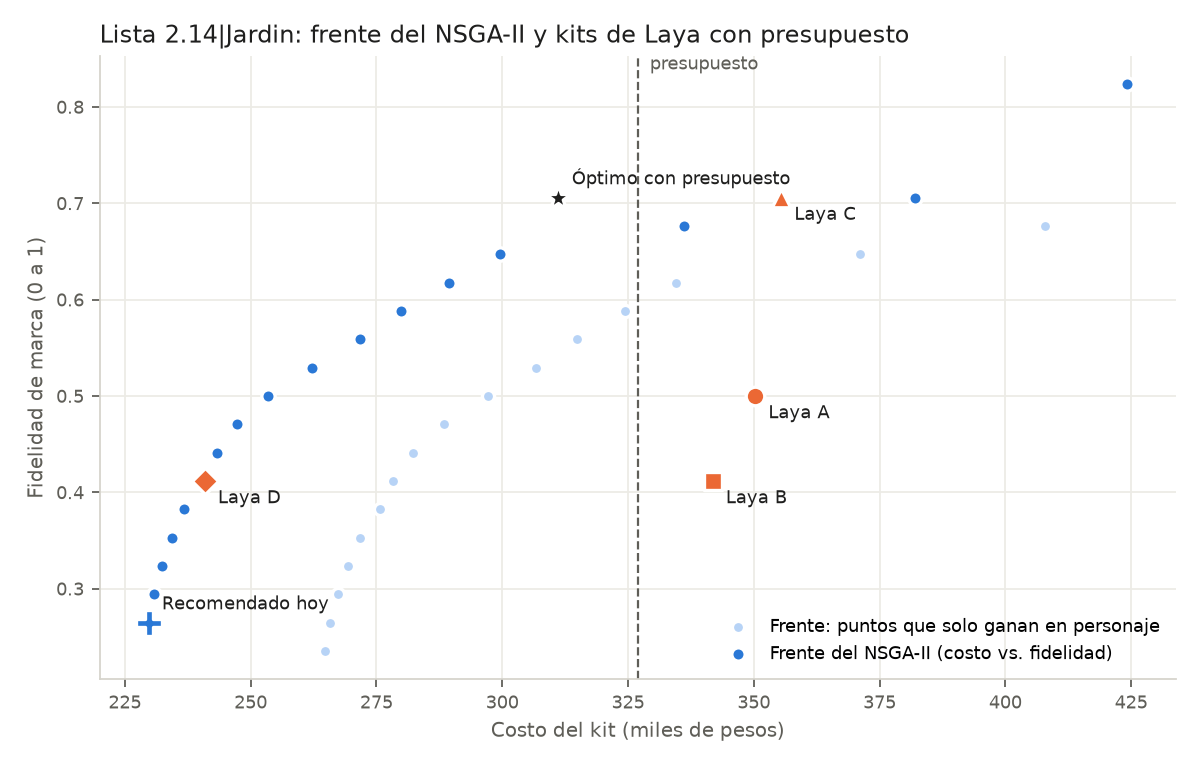
\includegraphics[width=0.88\textwidth]{../informes/benchmark-laya/fig_frente_2.14_Jardin.png}
\caption{Frente del NSGA-II proyectado en el plano costo-fidelidad para una
lista típica de 17 líneas. La cruz es el kit que se recomendaba en v3, el más
barato. Bajo la línea de presupuesto hay puntos del frente con fidelidad de
hasta 0,65, y el óptimo exacto (estrella, 0,70) queda por encima del frente,
lo que muestra que el frente es aproximado. Los puntos claros parecen
dominados en este plano, pero no lo están: ganan en el eje de personaje.
Los marcadores naranja son los kits del modelo de propósito general.}
\label{fig:frente-jardin}
\end{figure}

\subsection{Lectura de los resultados}

\begin{enumerate}
  \item \textbf{En los extremos, el NSGA-II es exacto, pero no es
        necesario.} Iguala el óptimo en el 100\,\% de los Premium y Fan y en el
        99,4\,\% de los Ahorrador promediando las cinco semillas. Es lo que
        predice el \cref{cor:extremos}: una regla línea por línea también es
        exacta. La regla simple fallaba el 20\,\% de los Ahorrador porque
        ordenaba por precio unitario (\cref{lem:precio-unitario}), y no por una
        limitación de las reglas voraces.
  \item \textbf{El aporte real del frente está en el compromiso.} Con
        presupuesto, el frente contenía kits que cabían y lograban el 94\,\%
        de la calidad posible, frente al 40\,\% del kit que se recomendaba. La
        diferencia no era de cómputo, porque el frente ya estaba calculado: la
        recomendación no lo usaba.
  \item \textbf{El frente es aproximado.} En el 68\,\% de las listas, la
        escalera de costo marginal dominaba algún punto del frente (en
        promedio el 5\,\% de sus puntos), lo que es coherente con el sesgo
        ordinal de los operadores (\cref{sec:opt-nsga}). Además, el óptimo
        exacto con presupuesto estaba por encima del mejor punto del frente en
        el 72\,\% de las listas.
  \item \textbf{Un modelo de decisión de propósito general no compite.} En sus
        modalidades línea por línea queda cerca del azar en Ahorrador y
        Premium: el sobrecosto medio es del 52\,\%, frente al 42,6\,\% del azar.
        Su prueba de cordura lo explica: acierta el 30\,\% de las preguntas
        «¿cuál es el más barato?» con entre 2 y 6 opciones, cuando el azar
        acierta el 31\,\%. Solo supera al azar cuando la respuesta consiste en
        encontrar una palabra (el personaje). Darle la lista completa lo
        empeora (en Fan baja del 92\,\% al 58\,\% de óptimos). Su mejor caso,
        juez entre kits (D), logra el 59\,\% de la calidad con presupuesto,
        pero ese resultado se debe sobre todo a los kits que se le entregan: un
        juez perfecto sobre los mismos kits llega al 93\,\%.
\end{enumerate}

\subsection{Efecto de las correcciones}

Las tres correcciones de la versión v4 (\cref{sec:opt-evolucion}) salieron
directamente de esta lectura. Repetida la evaluación con semilla 0 sobre las
mismas 174 listas:

\begin{table}[htbp]
\centering\small
\caption{Antes y después de las correcciones motivadas por la evaluación.}
\label{tab:antes-despues}
\begin{tabular}{@{}L{7.2cm}cc@{}}
\toprule
Métrica & v3 & v4 \\
\midrule
Regla simple: Ahorrador igual al óptimo & 80\,\% & 100\,\% \\
Listas en que la escalera domina algún punto del frente & 68\,\% & 0\,\% \\
Recomendado con presupuesto: calidad lograda & 40\,\% & igual al óptimo exacto \\
Recomendado con presupuesto: cabe en el tope & 100\,\% & 100\,\% \\
\bottomrule
\end{tabular}
\end{table}

La tercera fila requiere una precisión. Con presupuesto, la versión v4
recomienda el punto de mayor fidelidad del frente que cabe, y el frente ya
incluye los peldaños de la escalera. En estas instancias eso bastó para
alcanzar el óptimo exacto. El \cref{teo:mckp-poli} da una garantía que no
depende de la instancia: la programación dinámica alcanza el óptimo siempre.

\subsection{Reproducibilidad y tiempos}

Con cinco semillas, el NSGA-II entrega el mismo kit en el 94,5\,\% de las
listas en las que corre, y siempre en las que se enumeran. En las demás, el kit
cambia con la semilla; en el Ahorrador eso significa que en el 0,6\,\% de las
corridas el kit no es el más barato posible. Con la semilla fija que usa el
sistema, el resultado es determinista.

Los tiempos se midieron en 29 listas, en un proceso sin otras cargas, en una
CPU de 16 núcleos: 5,3~s de media, 6,3~s de mediana y 9,0~s de máximo para
producir \emph{todos} los kits de una lista. El modelo de propósito general en
una GPU portátil tarda entre 0,08 y 3,1~s por kit según la modalidad. Ninguno
de los dos tiempos limita el producto: son del mismo orden que leer una página
con el modelo multimodal.

\subsection{Limitaciones de la evaluación}

\begin{itemize}
  \item \textbf{Un hijo por lista.} La consolidación entre hermanos
        (\cref{sec:opt-lineas}) no entra en juego. Los hogares de varios hijos
        son el caso en que el acoplamiento podría aparecer.
  \item \textbf{Foto del catálogo a mitad de curaduría.} Con más candidatos
        por línea, el espacio crece y la calidad del frente puede cambiar.
  \item \textbf{Solo canal léxico.} Con el canal semántico, algunos renglones
        tendrían candidatos que aquí no tuvieron.
  \item \textbf{La fidelidad mide el nivel de marca}, no si el producto se
        parece a lo que escribió el colegio. Esa segunda dimensión es
        responsabilidad de la resolución y no se mide aquí.
  \item \textbf{Un solo tope de presupuesto.} El tope se fijó en la mitad del
        camino entre el Ahorrador y el Premium. Con otros topes, las cifras
        absolutas cambian.
\end{itemize}
